\begin{frame}
  \frametitle{\textbf{Charged Particle Suppression}}
  \begin{columns}
    \column{0.5\textwidth}
    \begin{itemize}
    \item Charged hadrons \textbf{heavily suppressed} in central collisions, but not in peripheral collisions
    \item Charged-hadron $R_{\text{AA}}$: measure of the suppression of charged hadrons in AA collisions as compared to pp collisions
    \end{itemize}
    \begin{align*}
      \boxed{R_{\text{AA}}^{\text{ch}} (p_{\text{T}}) = \cfrac{dN^{\text{AA}}_{\text{ch}} / dp_{\text{T}}}{\left< N_{\text{coll}} \right> dN^{\text{pp}}_{\text{ch}} / dp_{\text{T}}}}
    \end{align*}


    \begin{itemize}
    \item No suppression in small systems (pp, pPb)
    \item Colorless objects ($\gamma, W^{\pm}, Z$) are not suppressed
    \item Partons \textbf{lose energy via color interactions} as they traverse the QGP 
    \end{itemize}
    \column{0.5\textwidth}
    \begin{tikzpicture}
      \node{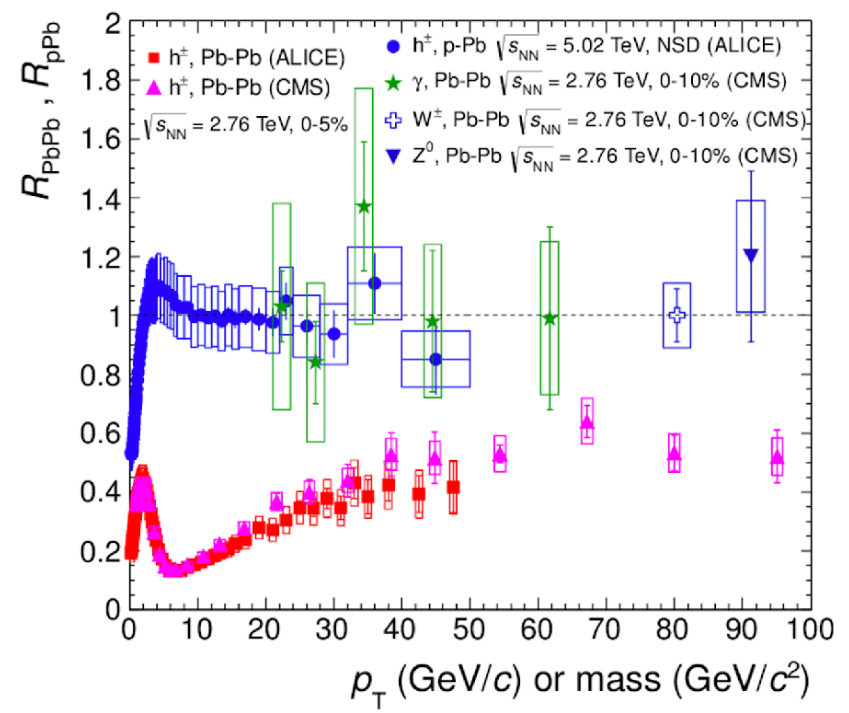
\includegraphics[width=\textwidth]{RAA-neutral-and-charged.png}};
      \node[font=\tiny] at (1.8,2.6) {\href{https://arxiv.org/abs/1012.1004}{arXiv:1012.1004}};
    \end{tikzpicture}
  \end{columns}
\end{frame}
